\section{Coloured Petri Nets}
\label{sect:language}

To present the concepts of CPNs, we use a CPN model of a distributed
two-phase commit transaction system. We use the example to give an
informal introduction to CPNs. The reader interested in the formal
definition of CPNs is referred to \cite{newcpnbook}.

% modules - substitution transitions

The CPN model of the two-phase commit system is comprised of 4
\concept{modules} hierarchically organized into three
levels. Figure~\ref{fig:commit} shows the top-level module which
consists of two \concept{substitution transitions} (drawn as
rectangles with double-lined borders) representing the
\figitem{Coordinator} and the \figitem{Workers} in the system. Each of
the substitution transitions has an associated \concept{submodule} that
model the behavior of the coordinator and the workers,
respectively. The name of the submodule is written in the rectangular
tag positioned at the bottom of each substitution transition.

\begin{figure}[b]
\centering
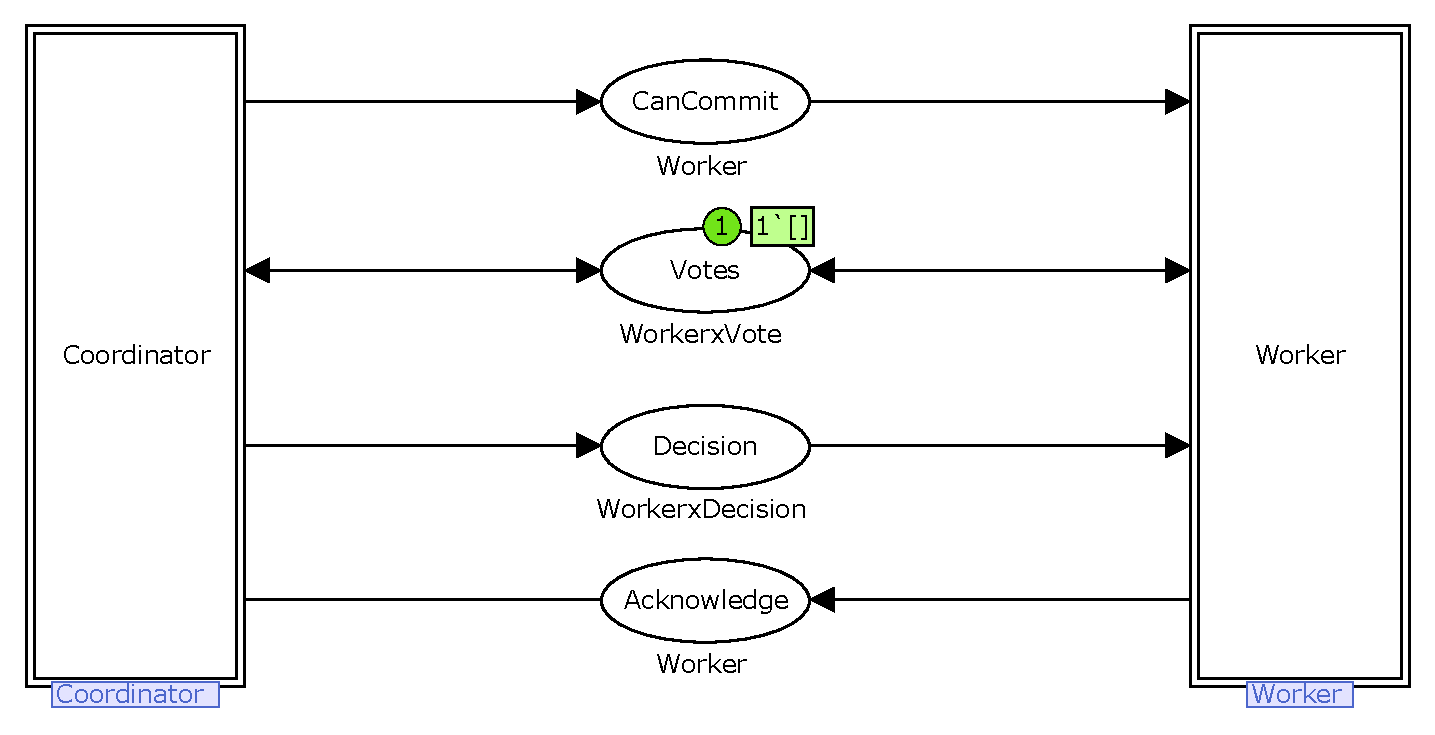
\includegraphics[scale=.52]{figures/Commit.eps}
\caption{The top-level module of the CPN model.}
\label{fig:commit}
\end{figure}

% places - tokens - colours - and colour sets

The two substitution transitions are connected via directed
\concept{arcs} to the four places \figitem{CanCommit},
\figitem{Votes}, \figitem{Decision}, and \figitem{Acknowledge} (drawn
as ellipses). Places connected to substitution transitions are called
\concept{socket places} and are linked to \concept{port} places on the
associated submodules (to be presented shortly). The coordinator and
the workers interact by producing and consuming \concept{tokens} on
the places. These tokens carry data values and the type of tokens that
may reside on a place is determined by the \concept{type} of the place
(written in text below the place). For historical reasons the types of
places are called \concept{color sets}. Figure~\ref{fig:coloursets}
lists the definitions of the color sets used for the four places in
Fig.~\ref{fig:commit}. These color sets are defined using the CPN ML
programming language.

The \smlcode{Worker} color set is an indexed type consisting of the
values \smlcode{wrk(1),wrk(2),...,wrk(W)} where the symbolic constant
\smlcode{W} is used to specify the number of worker processes
considered. This color set is used to model the identity of the worker
processes. The color set \smlcode{Vote} is an enumeration type
containing the values \smlcode{Yes} and \smlcode{No}, and is used to
model that a worker may vote \smlcode{Yes} or \smlcode{No} to commit
the transaction. The color set \smlcode{WorkerxVote} is a product type
containing pairs consisting of a worker and its vote. The color set
\smlcode{Decision} is an enumeration type used to model whether the
coordinator decides to \smlcode{abort} or \smlcode{commit} the
transaction (only if all workers vote yes will the transaction be
committed). It should be noted that in addition to the type
constructors introduced above, CPN ML supports union, lists, and
record types. The variables \smlcode{w} and \smlcode{vote} declared in
Fig.~\ref{fig:coloursets} will be introduced later.

\begin{figure}[]
\begin{verbatim}
val W = 2;

colset Worker = index wrk with  1..W;
colset Vote = with Yes | No;
colset WorkerxVote = product Worker * Vote;

colset Decision = with abort | commit;
colset WorkerxDecision = product Worker * Decision;

var w : Worker;
var vote : Vote;
\end{verbatim}
\caption{Definition of color sets used in Fig.~\ref{fig:commit}.}
\label{fig:coloursets}
\end{figure}


% marking - tokens initial marking - current marking

The state of a CPN model is called a \concept{marking}), and consists
of a distribution of \concept{tokens} on the places of the model. Each
place may hold a (possibly empty) \concept{multi-set} of tokens with
data values (colors) from the color set of the place. The
\concept{initial marking} of a place is specified above each place
(and omitted if the initial marking is the empty multi-set). For the
places in Fig.~\ref{fig:commit} all places are empty in the initial
marking. Initially, the \concept{current marking} of a CPN model
equals the initial marking. When a CPN model is executed occurrences of
enabled transitions consume and produce tokens on the places which
will change the \concept{current marking} of the CPN model.

 
% coordinator  - port places

The \figitem{Coordinator} module is shown in
Fig.~\ref{fig:coordinator}. This is the submodule associated with the
\figitem{Coordinator} substitution in Fig.~\ref{fig:commit}. The
places \figitem{CanCommit}, \figitem{Votes}, \figitem{Decision}, and
\figitem{Acknowledge} are \concept{port places} as indicated by the
rectangular \figitem{In} and \figitem{Out} tags positioned next to
them. These places are linked to the accordingly named places in the
top-level module (Fig.~\ref{fig:commit}) via a \concept{port-socket
  association} which implies that any tokens added (removed) from a
port place by transitions in the \figitem{Coordinator} module will
also be added (removed) in the marking of the associated socket place
in the top-level module. The places \figitem{Votes} and
\figitem{Acknowledge} are \concept{input port places} which means that
the module will only consume tokens from these places.  The places
\figitem{CanCommit} and \figitem{Decision} are \concept{output port
  places} which means that the \figitem{Coordinator} module will only
produce tokens on these places. It is also possible for a place to be
an input-output port place which means that the module may both
consume and produce tokens from (on) this place.

The places \figitem{Idle}, \figitem{WaitingVotes}, and
\figitem{WaitingAcknowledgement} are used to model the states that the
coordinator goes through when executing the two-phase commit
protocol. The places \figitem{Idle} and \figitem{WaitingVotes} have
the color set \smlcode{UNIT} containing just a single value
\smlcode{()} (denoted unit). Initially, the coordinator is in an idle
state as modeled by the initial marking of place \figitem{Idle} which
consists of a single token with the color unit. In CPN ML this
multi-set is written \smlcode{1`()} specifying one (\smlcode{1})
occurrence of (\smlcode{`}) the unit color (\smlcode{()}).  The number
of tokens on a place in the current marking is indicated with a small
circle positioned next to a place, and the detail of the color of the
tokens are provided in an associated text box. The indication of the
current marking of a place is omitted if currently the place contains
no tokens.

The transitions \figitem{SendCanCommit}, \figitem{CollectVotes}, and
\figitem{ReceiveAcknowledgements} model the events/actions that cause
the coordinator to change state. The coordinator will first send a can
commit message (transition \figitem{SendCanCommit}) to each worker
asking whether they can commit the transaction. Then the coordinator
will collect the votes from all workers (transition
\figitem{CollectVotes}) and send a decision to the workers that voted
yes indicating whether the transaction is to be committed or
not. Finally, the coordinator will receive an acknowledgment from each
worker that voted yes, confirming that they have received the decision
(transition \figitem{ReceiveAcknowledgements}).  It should be noted
that \figitem{CollectVotes} is a substitution transition which means
that the details of how the coordinator collects votes is modeled by
the associated \figitem{CollectVotes} submodule. This illustrates that
it is possible to mix the use of ordinary and substitution transitions
within a module. We do not describe the \figitem{CollectVotes} module
in this paper. The complete CPN model is available via \cite{cpnmodel}.

\begin{figure}[]
\centering
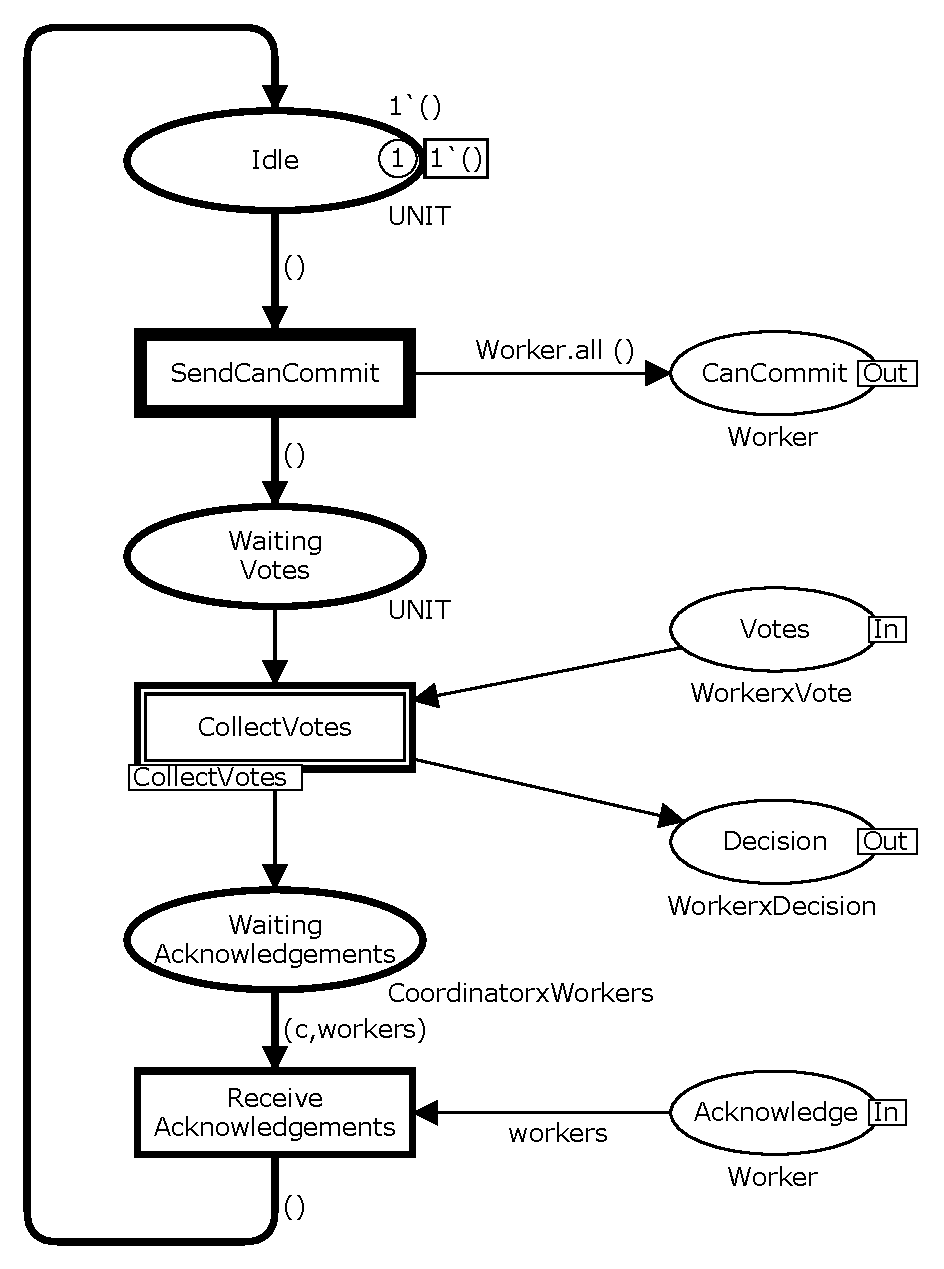
\includegraphics[scale=.5]{figures/Coordinator.eps}
\caption{The \figitem{Coordinator} module.}
\label{fig:coordinator}
\end{figure}


% basic enabling and occurrences

In the current marking shown in Fig.~\ref{fig:coordinator} only the
transition \figitem{SendCanCommit} is enabled as indicated by the
thick border of that transition. The requirement for a transition to
be \concept{enabled} is determined from the \concept{arc expressions}
associated with the incoming arcs of the transition. In this case,
there is only a single incoming arc from place \figitem{Idle}
containing the expression \smlcode{()}. This expression specifies that
for \figitem{SendCanCommit} to be enabled, there must be at least one
\smlcode{()}-token present on \smlcode{Idle}. When the
\smlcode{SendCanCommit} transition \concept{occurs}, it will consume a
\smlcode{()}-token from place \smlcode{Idle} and it will produce
tokens on places connected to output arcs as determined by evaluating
the arc expressions on output arcs. In this case, the expression
\smlcode{()} on the arc to \smlcode{WaitingVotes} evaluates to a
single \smlcode{()}-token. The expression \smlcode{Worker.all()} is a
call to the function \smlcode{Worker.all} that takes a unit value
(\smlcode{()}) as parameter and returns all colors of the color set
\smlcode{Worker}. This illustrates that it is very useful to be able
to hide complex calculations (e.g., of multi-sets of tokens or tokens
with complex data values) within function calls and to be able to
add/remove several tokens in a single step (transition occurrence)
without introducing a number of intermediate states (markings).

\ignore{
This illustrates that arc expression may also make
use of function to calculate the tokens to be added (removed) from
places. In particular this means that complex data manipulation can be
performed without intruding intermediate steps in the model itself.
}

Figure~\ref{fig:sendcancommit} shows the marking of the surrounding
places of transition \figitem{SendCanCommit} after the occurrence of
\figitem{SendCanCommit}. It can be seen that the place
\smlcode{CanCommit} contains two tokens - one of each worker in the
system - representing messages going to the two worker processes. The
coordinator has now entered a state in which it is waiting to collect
the votes from the worker processes.

\begin{figure}[h]
\centering
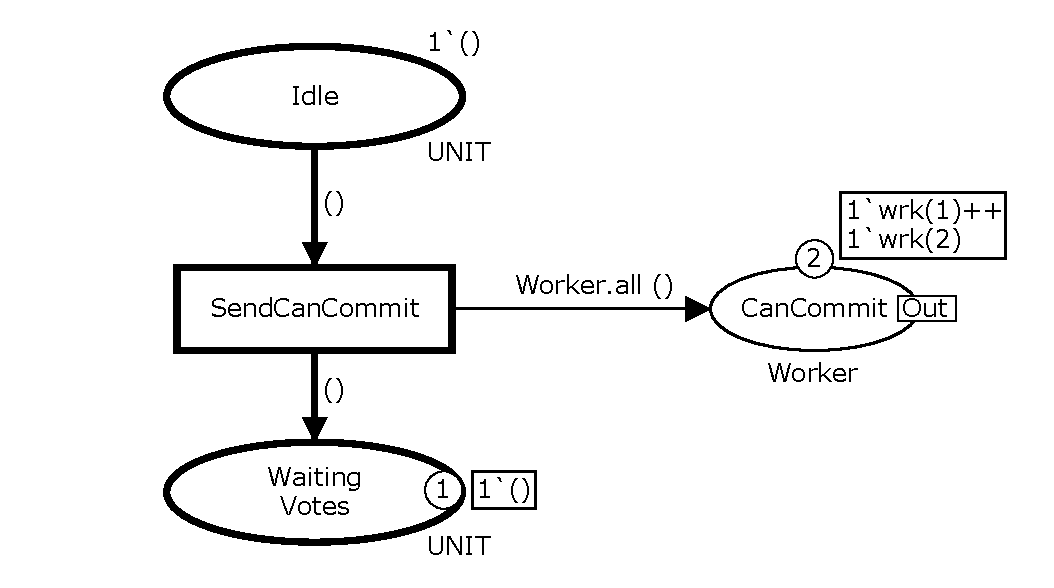
\includegraphics[scale=.5]{figures/SendCanCommit.eps}
\caption{Current marking after \figitem{SendCanCommit}.}
\label{fig:sendcancommit}
\end{figure}

% comparison to low-level nets

By setting the symbolic constant \smlcode{W} (see
Fig.~\ref{fig:coloursets}) we can easily configure the model to handle,
e.g., five workers. With ordinary Petri nets we would have had to
create a copy of the \figitem{CanCommit} place for each worker. In
particular, we would have to make changes to the net structure
(places, transitions, arcs) when changing the number of workers. This
shows that CPNs provides a means for easily creating parameterizable
models and also that it enables more compact modeling as we only need
a single instance of the \figitem{CanCommit} place in order to
accommodate any finite number of workers. 

\begin{itemize}
\item WE COULD EABORATE MORE ON THIS BY DRAWING THE CORRESPONDING
  PT-NET FOR THE CANCOMMIT TRANSITION. THAT WOULD ILLUSTRATE UNFOLDING
  OF PLACES (see comment at the end of this section that proposes
  illustration of unfolding transition. Perhaps it is a good approach
  to split the introduction of unfolding in two steps. Then at the end
  of the section we can mention that any CPNs can be unfolder to a
  possibly infinite behaviorally equivalent PT-nets. The two example
  that we have in this section would then nicely illustrate how. It
  would also be possible to factor this into a seperate section in
  order to avoid that this section becomes overlong in comparison with
  the other section.  
\end{itemize}

%\com{Maybe we could have shown
%  the corresponding fragment as a Place/Transition net? In this case we need more places - when we get to the worker we could also need to duplicate transition as per bindings}

% worker process - and binding and binding elements.

Figure~\ref{fig:worker} shows the \figitem{Worker} module which is the
submodule of the \figitem{Workers} substitution transition in
Fig.~\ref{fig:commit}. The places \figitem{CanCommit},
\figitem{Votes}, \figitem{Decision}, and \figitem{Acknowledge}
constitute the port places of this module and are linked to the
accordingly named socket places in Fig.~\ref{fig:commit}. The places
\figitem{Idle} and \figitem{WaitingDecision} models the two main
states of worker processes. Each of these places have the color set
\smlcode{Worker} and the idea is that when there is a token with color
\smlcode{wrk(i)} on, e.g., the place \figitem{Idle}, then this models
that the i'th worker is in state idle. This makes it possible to model
the state of all workers in a compact manner within a single module
without having to have a place for each worker or a module instance
for each worker. Initially, all workers are in the idle state as
represented by corresponding tokens on place \figitem{Idle} in the
initial marking. The transition \figitem{ReceiveCanCommit} models the
reception of can commit messages from the coordinator and the sending
of a vote. The transition \figitem{ReceiveDecision} models the
reception of a decision message from the coordinator and the sending
of an acknowledgment.

\begin{figure}[]
\centering
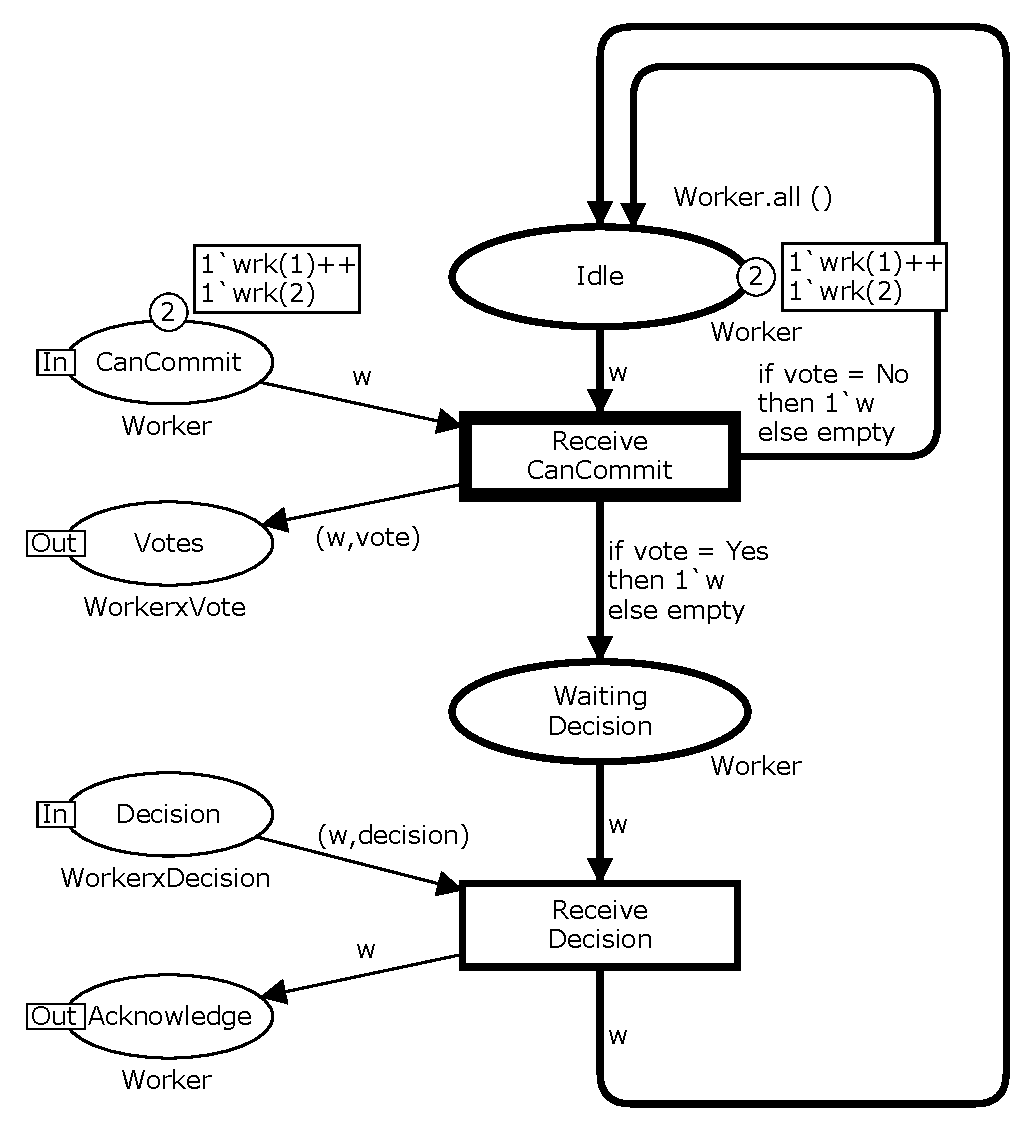
\includegraphics[scale=.5]{figures/Workers.eps}
\caption{The \figitem{Worker} module.}
\label{fig:worker}
\end{figure}

The current marking of place \figitem{CanCommit} is \smlcode{1`wrk(1)
  ++ 1`wrk(2)} modelling a marking where the coordinator has sent a
can commit message to each worker. The thick border of transition
\figitem{ReceiveCanCommit} indicates that this transition is enabled
in the current marking. The arc expressions on the surrounding arcs of
the \figitem{ReceiveCanCommit} transition are more complex than the
arc expressions of the \figitem{SendCanCommit} transition in the
\figitem{Coordinator} module considered earlier in that they contain
the \smlcode{free variables} \smlcode{w} and \smlcode{vote} defined in
Fig.~\ref{fig:coloursets}. This means that in order to talk about the
enabling and occurrence of transition \smlcode{ReceiveCanCommit}, we
need to assign values to these variables in order to evaluate the
input and output arc expressions. This is done by creating a
\concept{binding} which associates a value to each of the free
variables occurring in the arc expression of the transition. Bindings
can be considered different modes in which a transition may occur.  As
\smlcode{w} is of type \smlcode{Worker} and \smlcode{vote} is of type
\smlcode{Decision}, this gives the following four possible bindings
reflecting that each of the two workers may vote yes or no to
committing the transactions:

\begin{eqnarray*}
b_{1Y} & = & \langle \smlcode{w} = \smlcode{wrk(1)}, \smlcode{vote} = \smlcode{Yes} \rangle \\
b_{1N} & = & \langle \smlcode{w} = \smlcode{wrk(1)}, \smlcode{vote} = \smlcode{No} \rangle \\
b_{2Y} & = & \langle \smlcode{w} = \smlcode{wrk(2)}, \smlcode{vote} = \smlcode{Yes} \rangle \\
b_{2N} & = & \langle \smlcode{w} = \smlcode{wrk(2)}, \smlcode{vote} = \smlcode{No} \rangle
\end{eqnarray*}

A binding of a transition is enabled if evaluating each input arc
expression in the binding results in a multi-set of tokens which is a
subset of the multi-set of tokens present on the corresponding input
place. For an example, consider the binding $b_{1Y}$. Evaluating the
input arc expression \smlcode{w} on the input arc from \smlcode{Idle}
results in the multi-set containing a single token with the color
\smlcode{wrk(1)} which is contained in the multi-set of tokens present
on place \figitem{Idle} in the marking depicted in
Fig.~\ref{fig:worker}. Similarly for the input arc expression on the
arc from place \figitem{CanCommit}. This means that binding $b_{1Y}$
is enabled and may occur. In fact, all four bindings listed above
is enabled in the marking shown in Fig.~\ref{fig:commit}.

% ocurrence and more complicated evaluation

The tokens produced on output places when a transition occurs in an
enabled binding is determined by evaluating the output arc expressions
of the transition in the given binding. Consider again the binding
element $b_{1Y}$. The output arc expression \smlcode{(w,vote)} will
evaluate to \smlcode{(wrk(1),Yes)} and this token will be added to
place \smlcode{Votes} to inform the coordinator that worker 1 votes
yes to committing the transaction. The arc expression on the arc from
\figitem{ReceiveCanCommit} to \figitem{WaitingDecision} is an
if-then-else expression which in the binding $b_{1Y}$ will evaluate to
the multi-set $1`wrk(1)$ which will be added to the tokens on place
\figitem{Waiting}. The if-then-else expression on the arc from
\figitem{ReceiveCanCommit} to \figitem{Idle} evaluates to the
\smlcode{empty} multi-set and hence no tokens will be added to place
\figitem{Idle} in this case. Figure~\ref{fig:receivecancommit} shows
the marking resulting from an occurrence of the $b_{1Y}$ binding.

\begin{figure}[h]
\centering
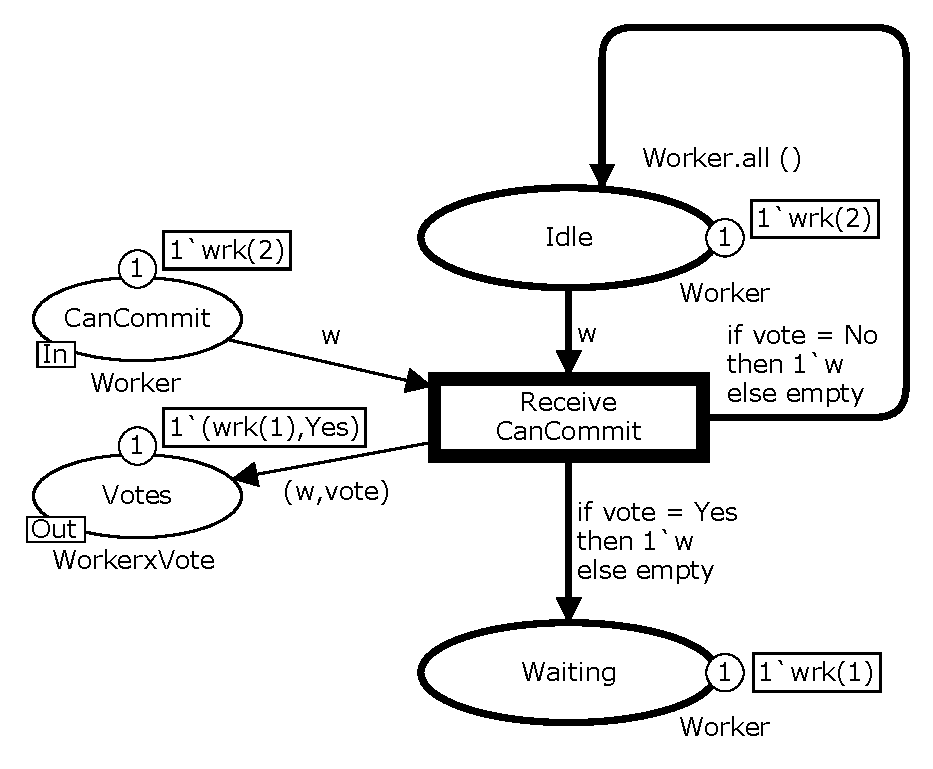
\includegraphics[scale=.5]{figures/ReceiveCanCommit.eps}
\caption{Current marking after occurrence of \figitem{ReceiveCanCommit}.}
\label{fig:receivecancommit}
\end{figure}

The occurrence of the binding $b_{1N}$ representing that worker one
votes no would have the effect of removing a \smlcode{wrk(1)}-token
from \figitem{Idle}, adding a \smlcode{(wrk(1),No)}-token to
\figitem{Votes}, and adding no tokens to place
\figitem{WaitingDecision} and adding a \smlcode{wrk(1)}-token to place
\figitem{Idle}. This models the fact that if a worker votes no to
committing the transaction, then it goes back to idle; whereas if it
votes yes, then it will go to waiting to be informed about whether the
transaction is to be committed or not.  Recall that this is a
distributed system and hence a worker cannot (without exchanging
messages) know what other workers have voted.  Above we have
considered relatively simple arc expressions but the arc expressions
of a transition can be any expression that can be written in Standard
ML as long as they have types that matches the corresponding
places. In particular, arc expressions may apply functions including
higher-order functions.

All four bindings listed for transition \figitem{ReceiveCanCommit}
were enabled in the marking shown in
Fig.~\ref{fig:worker}. Furthermore, enabled bindings may be
\concept{concurrently enabled} if each binding can get its required
multi-set of tokens from each input place independently of the other
enabled bindings in the set. As an example, the two bindings $b_{1Y}$
and $b_{2Y}$ are concurrent enabled since each binding can gets its
token from the input places without sharing with each other. This
reflects that the workers are executing concurrently and may
simultaneously send a vote back to the coordinator. In contrast, the
two bindings $b_{1Y}$ and $b_{1N}$ are not concurrently enabled. These
two bindings are in \concept{conflict} because they each need the
single \smlcode{wrk(1)}-token on \figitem{Idle} (and in fact also the
single \smlcode{wrk(1)}-token on place \figitem{CanCommit}. The notion
of concurrency and conflict of binding extends to bindings of
different transitions. A fundamental property of a set of concurrently
enabled bindings that CPNs inherit from Petri nets is that theses can
be executed in any interleaved order and the resulting marking will be
the same independently of the interleaved execution considered.

\begin{itemize}

\item HERE WE COULD MAKE A FURTHER LINK TO PT-NETS BY SHOWING THE
  FRAGMENT CORRESPONDING TO RECEIVECANCOMMIT. THAT WOULD ILLUSTRATE
  UNFOLDING OF TRANSITIONS.

\item HERE WE COULD BRIEFLY MENTION GUARDS. 

\item WE COULD BRIEFLY TALK ABOUT MODELING TIME IF WE SKIP HAVING
  A SECTION ON THIS.

\end{itemize}
